\section{Implementierung}
\label{sec:implementierung}

\subsection{Implementierung der Prozessplanung}
\label{subsec:prozessplanung_implementierung}

Für die Implementierung gilt es nun zunächst eine Grundlage zu finden, welche die zuvor genannten Kriterien erfüllt. Der Vollständigkeit halber seien hier noch einmal alle Kriterien aufgelistet:
%
\begin{compactenum}[1.]
    \item Simplizität
    \item Vielschichtigkeit
    \item Intuitivität
    \item Zugängliche Plattform
    \item JavaScript
    \item Touchoptimiert
    \item Dezentralisierung
    \item Virtualisierung
    \item Interoperabilität
    \item Serviceorientierung
    \item Modularität
    \item Echtzeitfähigkeit
\end{compactenum}

Um komplexe Prozesse auch für Laien zugänglich zu machen, bietet sich ein visuelles Interface an. Ein textbasiertes Interface wäre hierfür zu komplex und eine auf Knöpfen und Formularelementen basierende Oberfläche wäre nicht skalierbar genug.\\
Eine Benutzeroberfläche ähnlich der von Scratch kommt in den Sinn [\cite{scratchInterface}], und tatsächlich gibt es von Google die clientseitige Bibliothek „Blockly“, welche auch in Applikationen wie Google Coding School, Code.org, oder Hour of Code genutzt wird. Weitere wesentliche Gründe für die Verwendung von Blockly sind die Design-Kriterien des Frameworks. So erfüllt Blockly viele der genannten Kriterien wie Simplizität, Intuitivität, Touchoptimierung, etc.\\
Blockly bietet einen Editor, welcher benutzt werden kann, um mithilfe von ineinandergreifenden, Puzzle-artigen Blöcken über das drag\&drop-Prinzip Code-Konzepte darzustellen. Dieser Editor ist in Grafik \ref{fig:blocklyOverview} abgebildet.
%
\begin{figure}[htbp]
	\centering\includegraphics[width=1.0\textwidth]{images/04/Blockly_Overview.eps}
    \caption{Googles Blockly Editor}
    \label{fig:blocklyOverview}
\end{figure}

Die so abgebildete Logik kann dann in Form einer beliebigen Programmiersprache ausgegeben werden. Das Wesentliche ist jedoch Blocklys Erweiterbarkeit und Anpassungsfähigkeit. So ist es möglich, neue „Blöcke“ zu definieren und ihnen eine selbst definierte Logik zuweisen. Da diese Blöcke während der Initialisierung des Editors als Konfiguration übergeben werden können, ist es des Weiteren möglich, eine Konfiguration automatisiert zu generieren. So kann eine Sammlung an Blöcken (und damit Funktionsbausteinen) dynamisch für die verfügbaren Anlagen und deren Funktionen generiert werden.

So lassen sich also Blöcke für die Aktivierung und Deaktivierung aller Aktoren aller registrierter PLCs automatisch generieren. Zusätzlich dazu können noch einige generische und logische Blöcke wie Schleifen hinzugefügt werden. Daraus resultiert ein Editor, welcher wie in Grafik \ref{fig:MBOMGen_Config} auf der linken Seite eine Kategorie für jede PLC hat und darin die dazugehörigen Blöcke.
%
\begin{figure}[htbp]
	\centering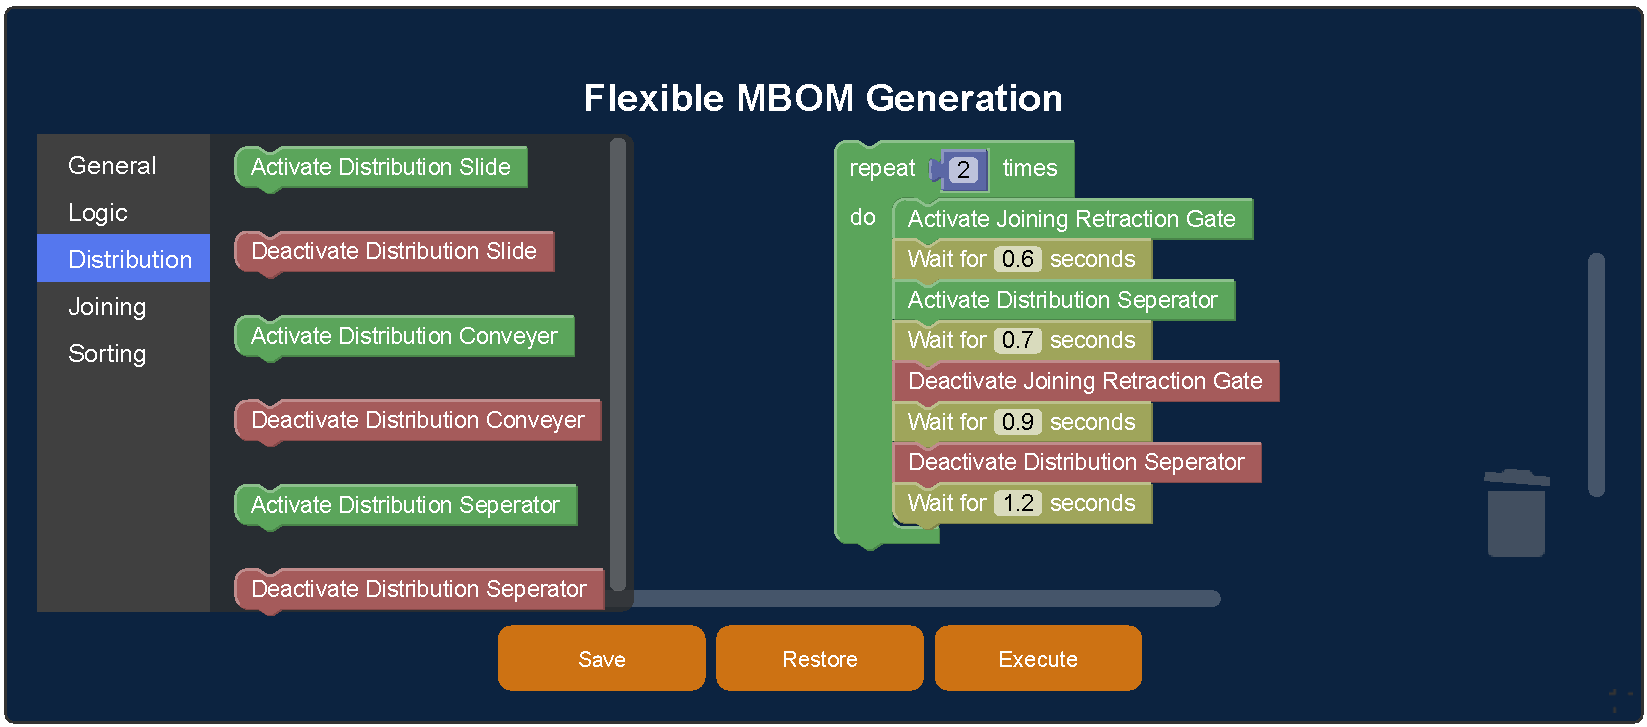
\includegraphics[width=1.0\textwidth]{images/04/MBOMGen_Config.pdf}
    \caption{Implementierter Editor mit ausgeklappter Toolbar}
    \label{fig:MBOMGen_Config}
\end{figure}

Wie ebenfalls in Grafik \ref{fig:MBOMGen_Config} zu sehen ist, lassen sich diese Blöcke über drag\&drop aus der Toolbar (der Sammlung von Blöcken auf der linken Seite) in den Arbeitsbereich (dem scrollbaren Bereich auf der rechten Seite) ziehen. Dort greifen die Blöcke ineinander, was mit dem Nutzer in Form von visuellen und akustischen Hinweisen kommuniziert wird. Welche Blöcke wie ineinandergreifen können, ist außerdem direkt anhand der Zähne zu erkennen, während die Farbe der Blöcke über den Typ Blockes aufklärt. So sind etwa Aktivierungsblöcke grün und Deaktivierungsblöcke rot.

Neben diesen Blöcken zur Steuerung der Aktoren gibt es auch Böcke für allgemeine Funktionen wie etwa zum Warten oder Loggen, elementare Blöcke für Zahlen oder Strings, logische Blöcke für Schleifen oder (konzeptuelle) Bedingungen, und boolesche Blöcke für den Status eines Aktuators. Ein solcher logischer Block ist etwa in Grafik \ref{fig:MBOMGen_Conditional} abgebildet.
%
\begin{figure}[htbp]
	\centering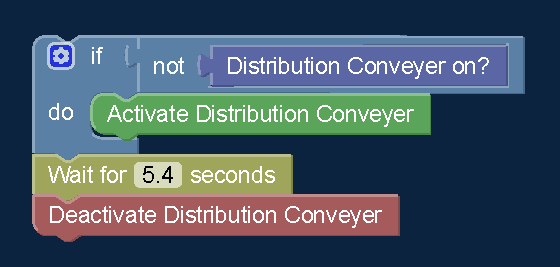
\includegraphics[width=0.6\textwidth]{images/04/MBOMGen_Conditional.pdf}
    \caption{Beispiel eines Logik-Blocks}
    \label{fig:MBOMGen_Conditional}
\end{figure}

Zudem wurde eine Speicherungs- und Wiederherstellungs-Funktion hinzugefügt, welche es jedem Nutzer der Webseite ermöglicht, seinen aktuellen Arbeitsbereich exakt abzuspeichern und ihn jederzeit wiederherzustellen. Um einen Prozess zu speichern, wird dieser zu XML konvertiert und dieser XML Code wird dann als String abgespeichert. Wo genau diese Daten abgespeichert und übermittelt werden und wie die Authentifizierung funktioniert, wird im Folgenden in Kapitel \ref{subsec:prozesssteuerung_architektur} behandelt.

Neben dem Prozess-Editor wurde zudem noch ein Fenster für einen Live-Videostream der Anlage eingefügt, sodass ein Nutzer in nahezu Echtzeit die Ausführung des Prozesses auf der echten Anlage beobachten kann. Außerdem wurde ein Graph eingefügt, welcher den aktuellen Status aller Aktuatoren dieser Anlage anzeigt. Diese beiden Blöcke sind in Grafik \ref{fig:MBOMGen_AllBlocks} abgebildet. Im Anhang dieser Arbeit unter \ref{lst:anhang_code_xml} lässt sich zudem der XML Code eines simplen Prozesses finden.
%
\begin{figure}[htbp]
	\centering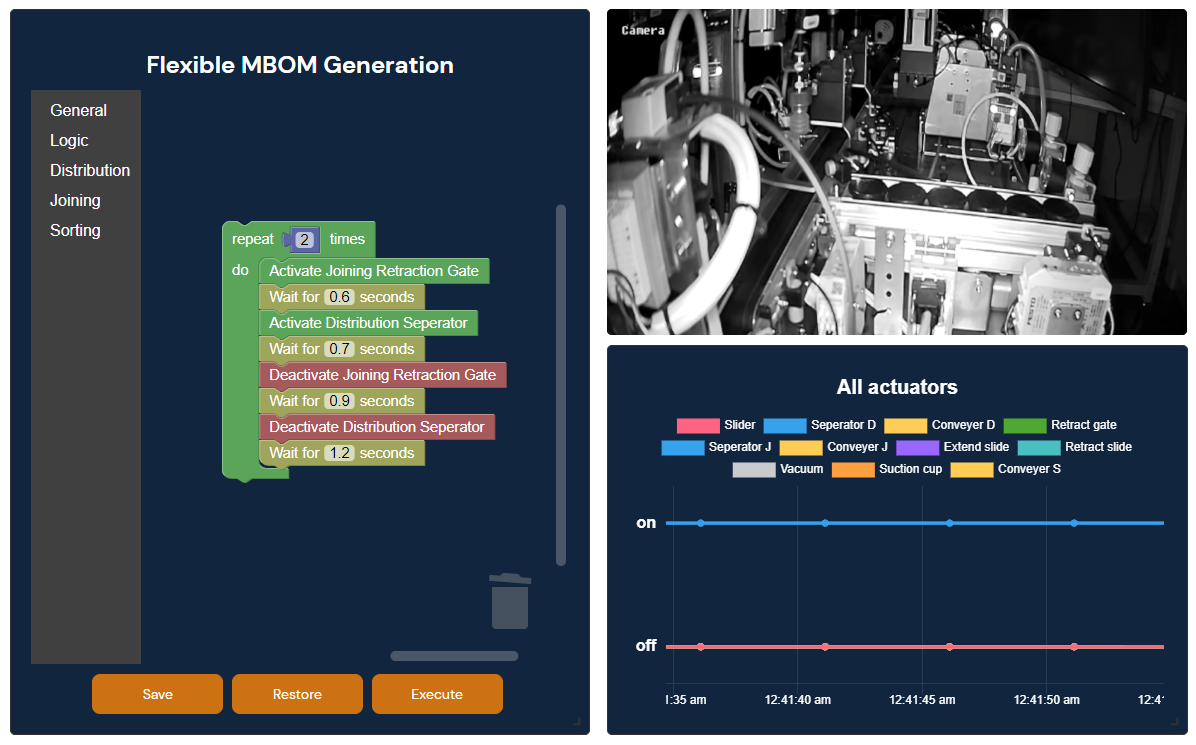
\includegraphics[width=1.0\textwidth]{images/04/MBOMGen_AllBlocks.png}
    \caption{Aufbau der Prozessplanungs-Seite}
    \label{fig:MBOMGen_AllBlocks}
\end{figure}

\subsubsection{Übersichtsseite}
\label{subsubsec:prozessplanung_implementation_übersichtsseite}

Neben der „Flexible MBOM Generation“ Seite wurde auch eine „MBOM Overview“ Seite angelegt, welche es ermöglicht, die gespeicherten Prozesse aller Nutzer anzuzeigen und Metriken zu ihnen zu berechnen. Dies erklärt auch die Benennung der Seiten: „MBOM“ steht für „Manufacturing bill of materials“ und repräsentiert eine Liste, welche alle erforderlichen Teile und Baugruppen enthält, die benötigt werden, um ein vollständiges Produkt anzufertigen. Der geplante Prozess enthält dabei theoretisch alle benötigten Informationen, wie etwa die verbrauchten Ressourcen, jedoch ist es recht umständlich, diese Daten aus den Blöcken abzulesen. Die Übersichtsseite erleichtert diese Aufgabe, indem der Prozessplan analysiert und alle relevanten Informationen übersichtlich präsentiert werden. In Grafik \ref{fig:MBOMOverview} ist diese Seite abgebildet. Wie dort zu sehen ist, kann oben ein Prozessplan ausgewählt werden, welcher dann links angezeigt wird; auf der rechten Seite werden dann die relevanten extrahierten Daten zu diesem Prozessplan angezeigt.
%
\begin{figure}[htbp]
	\centering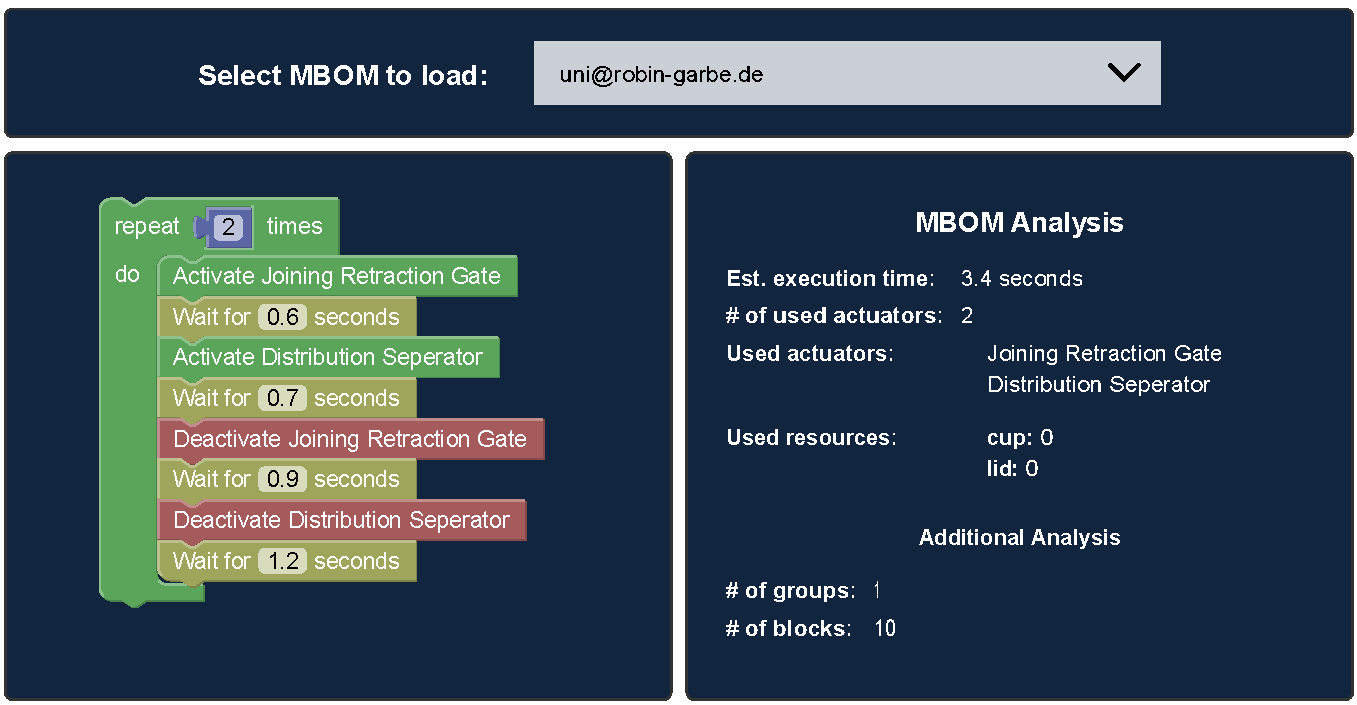
\includegraphics[width=1.0\textwidth]{images/04/MBOMOverview.pdf}
    \caption{Prozessplanungs-Übersichtsseite}
    \label{fig:MBOMOverview}
\end{figure}

Um diese Informationen zu extrahieren, wird der XML String des Prozesses untersucht und ein JavaScript Objekt mit den relevanten Daten wird erstellt. Dieses Objekt wird dann genutzt, um die erwähnten Informationen anzuzeigen. Der Code, um dieses Objekt zu erstellen, kann im Anhang unter \ref{lst:anhang_code_analyse} gefunden werden.

\subsection{Implementierung der Prozesssteuerung}
\label{subsec:prozesssteuerung_implementierung}

Die Cloud-Schicht mit simpler REST API und Datenbank besteht bereits und wird bei AWS gehostet. Die API ist mit C\# geschrieben und für die Datenbank wird eine manuell installierte MariaDB Datenbank genutzt. Das C\# Programm umfasst noch eine Vielzahl zusätzlicher Module, wie etwa für MQTT, OPC, Rest Connection, VPN-Server, DNS-Server und einige weitere.

Die Authentifizierung wird auf der Digital Twin Academy Webseite zentral geregelt und der API-Key wird in dem lokalen Speicher des Web-Browsers – konkreter in dessen „SessionStorage“ – abgelegt und nach dem Schließen des Browsertabs werden diese Daten automatisiert gelöscht. So wird eine clientseitige Datenspeicherung konform zu den EU Regulationen und den aufgeführten Sicherheitsstandards erreicht.\\
ES11 hat Zugriff auf die \verb|fetch| Browser-API, welche genutzt werden kann, um mithilfe von JavaScript eine Anfrage an die REST API zu senden. Des Weiteren unterstützt ES11 \verb|async| Funktionen, welche genutzt werden können, um die \verb|fetch| Anfragen asynchron abzuhandeln. In Blockly kann jedem Block Code in String-Form zugeordnet werden. Wenn dann das Blockly „Programm“ zu Code exportiert werden soll, werden diese String einfach entsprechend der definierten Logik konkateniert. Das Resultat ist ein Skript als String, welches dann vom Browser geparst und ausgeführt werden kann. Jeder Aktivierungs- oder Deaktivierungs-Block führt also letztlich eine \verb|fetch| Anfrage an die API aus. Die API prüft die Validität des API-Keys und ob die Aktion gültig ist; so dies der Fall ist, wird der geänderte Status des Aktuators in der Datenbank vermerkt und über den integrierten OPC-UA Client wird die Anfrage direkt an die entsprechende PLC weitergegeben.

Im Folgenden ist das JavaScript Object angegeben, welches einen Block konfiguriert. Hier sei beispielhaft der häufig verwendetet \verb|instruction_wait| angeben, welcher die Ausführung für die angegebene Anzahl an Sekunden anhält.

\begin{lstlisting}[language=JavaScript]
{
	"type": "instruction_wait",
	"message0": "Wait for %1 seconds",
	"args0": [
		{
			"type": "field_number",
			"name": "wait_amount",
			"value": 1,
			"min": 0,
			"max": 600,
			"precision": 0.1
		}
	],
	"previousStatement": null,
	"nextStatement": null,
	"colour": 65,
	"tooltip": "",
	"helpUrl": ""
}
\end{lstlisting}

Diesem Block kann nun mit dem folgenden Code Funktionalität zugewiesen werden. Diese Funktion wird auch „Block Generator“ genannt. Wie bereits erwähnt, wird der zugewiesene Code in Form eines Strings übergeben.

\begin{lstlisting}[language=JavaScript]
Blockly.JavaScript['instruction_wait'] = function(block) {
	var number_wait_amount = block.getFieldValue('wait_amount');
	var code = `await new Promise(resolve => setTimeout(resolve, ${Number(number_wait_amount) * 1000}));\n`;
	return code;
};
\end{lstlisting}

Das Programm nimmt sich also den API-Key aus der SessionStorage, stellt damit eine \verb|fetch| Anfrage an die API in der Cloud, um alle nötigen Informationen zu den verfügbaren PLCs und Aktoren einzusammeln, um damit dann den Editor für die Prozessplanung zu erstellen. Wird eine Prozessplanung ausgeführt, so wird das Prozesssteuerungs-Skript generiert, geparst und ausgeführt.

Die HTTP \verb|POST| Methode wird verwendet, um Daten ohne Rückgabewert an die API zu senden und die \verb|GET| Methode wird genutzt, um Daten abzurufen. Im Folgenden sei etwa der Code der selbst-aufrufenden, asynchronen Pfeilfunktion für \verb|POST| Anfragen aufgeführt. \verb|endpoint| stellt dabei die (Teil-)Adresse für den anzusteuernden Aktuator dar und wird übergeben. \verb|api_key| ist der aus der SessionStorage ausgelesene API-Key.

\begin{lstlisting}[language=JavaScript]
(async () => {
  const url = "https://digitaltwinservice.de/api/Database/" + endpoint;
  const response = await fetch(url, {
    method: "POST",
    headers: {
      "X-API-KEY": api_key,
      "accept": "/"
    }
  })
  .then(resp => resp.status);
  console.log("%cResponse status: " + response, "background:#5C4084bb;color:white;padding:1px 4px 1px 16px;border-radius:2px;");
  return response;
})()
\end{lstlisting}

Der beschriebene Ausführungsmodus wird als „direct“ bezeichnet. Neben diesem Ausführungsmodus wurde auch der „virtual“ Modus angelegt, welcher dafür gedacht ist, anstelle der echten Anlage eine virtualisierte Anlage anzusteuern. Hierauf wird in Kapitel \ref{cha:verifikation} näher eingegangen.

Nun sei noch ein Ablaufplan für die Kommunikation zwischen den drei Schichten für eine typische Prozessplanung und -steuerung in Grafik \ref{fig:dtaProzessAblaufplan} abgebildet.
%
\begin{figure}[htbp]
	\centering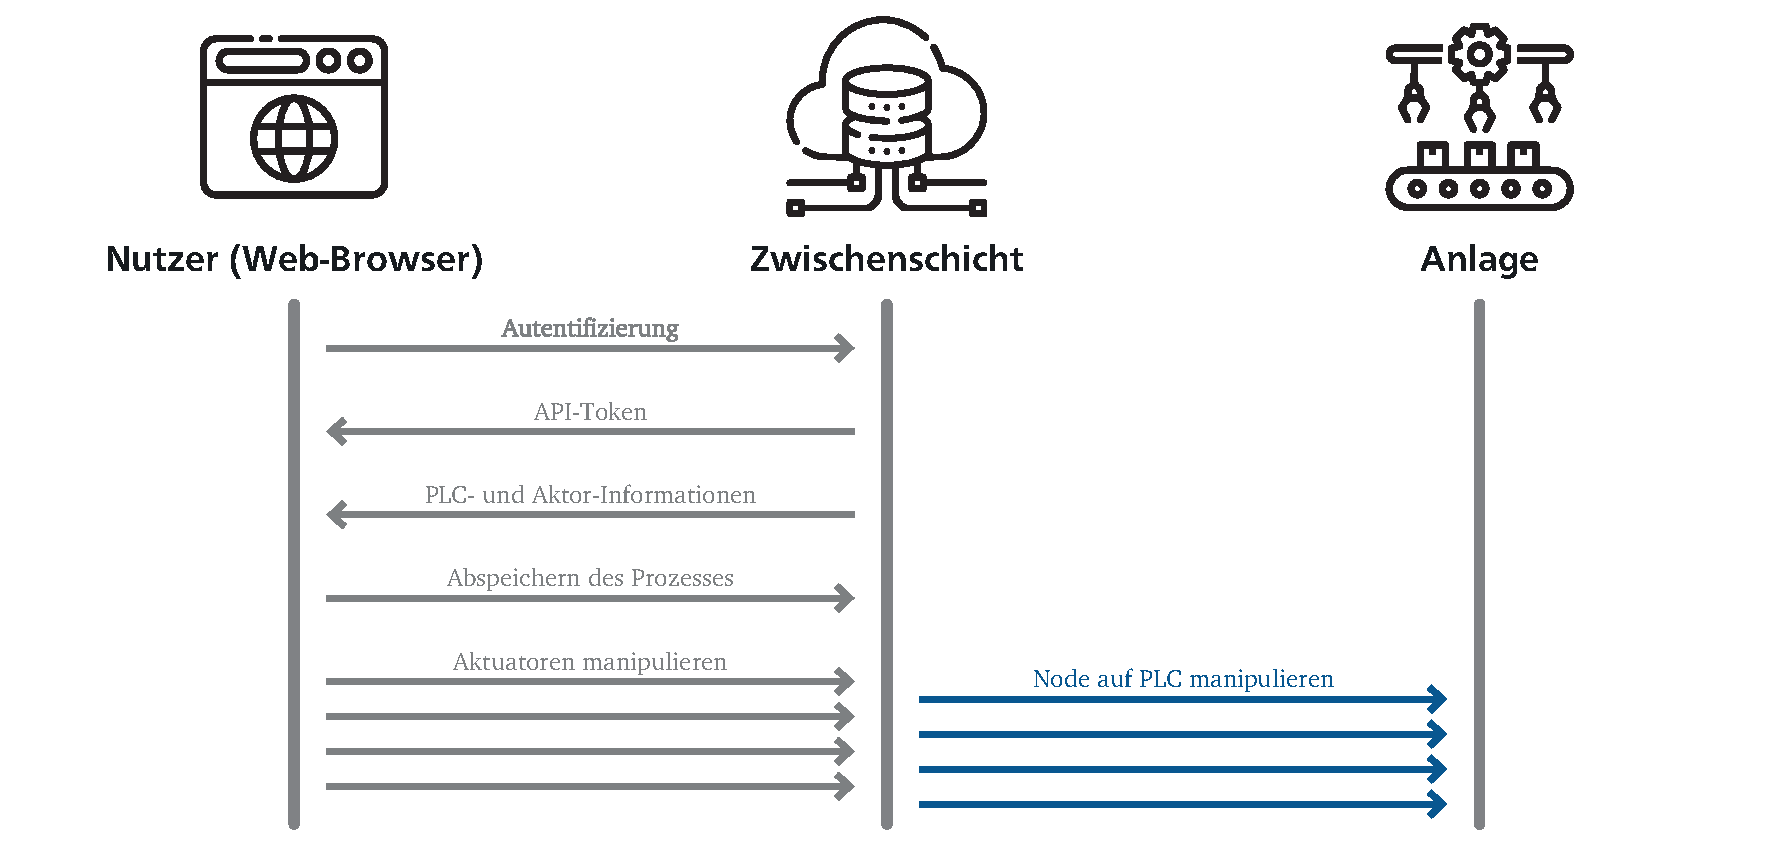
\includegraphics[width=1.0\textwidth]{images/04/dtaProzessAblaufplan.eps}
    \caption{Ablaufplan einer Prozessplanung und -steuerung}
    \label{fig:dtaProzessAblaufplan}
\end{figure}

\subsection{Implementierung der Produktionsplanung}
\label{subsec:produktionsplanung_implementierung}

Die Implementierung der Produktionsplanung läuft in großen Teilen analog zur Prozessplanung und sei hier nur kurz angeschnitten. In Grafik \ref{fig:produktionsplanung} ist die erstellte Benutzeroberfläche für die Produktionsplanung abgebildet. Jede Maschine wird als eigene Zeile dargestellt und jeder Auftrag wird als Block abgebildet. Die Breite eines Blockes repräsentiert dessen Ausführungsdauer, während die Farbe für die Art des Blockes steht. Die „Art“ bezeichnet hier eine Produktkonfiguration, wobei vorgesehen ist, dass jede Maschine nur eine Art von Produktkonfigurationen anfertigen kann. Jedoch soll eine Maschine umgerüstet werden können, sodass um andere Konfigurationen anfertigen zu können.
%
\begin{figure}[htbp]
	\centering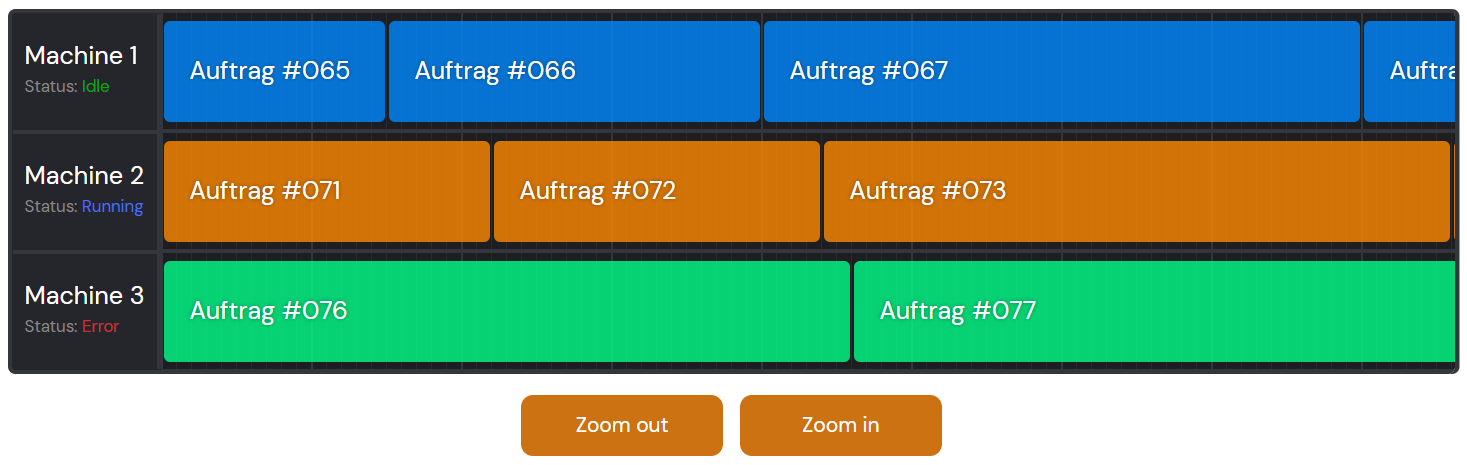
\includegraphics[width=1.0\textwidth]{images/05/Produktionsplanungs.png}
    \caption{Benutzeroberfläche der Produktionsplanung}
    \label{fig:produktionsplanung}
\end{figure}

Es sei jedoch erwähnt, dass diese Anwendung hier nur konzeptionell umgesetzt wird, da es zum aktuellen Zeitpunkt noch keine Möglichkeit gibt, diese Produktionsplanung an den bestehenden Produktionsablauf anzubinden. Dies liegt neben dem Fehlen von mehreren und unterschiedlichen Anlagen vorwiegend an der Art der Planung. Für eine Demo- und Bildungs-Webseite wie Digital Twin Academy wäre es wenig sinnvoll, wenn alle geplanten Prozesse erst in den kommenden Tagen ausgeführt werden; stattdessen sollten die Prozesse möglichst zeitnah an die Anlage weitergeben werden. Zudem werden bei der aktuellen Architektur die PLCs der Anlagen direkt angesteuert, was eine Lastenverteilung über mehrere Anlagen hinweg wenig sinnvoll macht. Zuletzt rechtfertigt die aktuelle und auch die auf kurze Sicht vorhergesehene Menge an auszuführenden Prozessen eine so komplexe Produktionsplanung nicht. Anders als die in Kapitel \ref{cha:prozessplanungUndProzesssteuerung} betrachtete endbenutzergesteuerte Prozessplanung und -steuerung wird hier also das theoretische Potenzial einer automatisierten und anpassbaren Produktionsplanung im Kontext von Industrie 4.0 im Allgemeinen untersucht.
